% \documentclass[12pt, handout]{beamer}
\documentclass[12pt, aspectratio=169]{beamer}

\usetheme{moloch}
\molochset{block=fill}

\usepackage{fontspec}
\setsansfont[
    UprightFont = Inter-Light,          % Use light as the normal font weight
    BoldFont = Inter-SemiBold,           % Use semibold for \textbf
    ItalicFont = Inter-LightItalic,      % Light italic for \textit
    BoldItalicFont = Inter-SemiBoldItalic % Semibold italic for \textbf with \textit
]{Inter}[RawFeature={+ss04, +ss03, +dlig, +tnum}]
% Inter font stylistic sets:
% ss01: alternate digits for 3, 4, 6, 8
% ss02: for disambiguation (with zero) in places like "Ill" or "O0" etc
% ss04: for disambiguation (without zero) in places like "Ill" etc
% ss03: round comma, quation marks

\usepackage{upquote}
\usepackage{microtype}
\UseMicrotypeSet[protrusion]{basicmath}    % disable protrusion for tt fonts

\usepackage{amsmath}
\usepackage{amssymb}
\usepackage{unicode-math}
\setmathfont{Erewhon Math}[Scale=1.14]

\usepackage{hyperref}
\pdfstringdefDisableCommands{\def\translate#1{#1}}
\usepackage{bookmark}
\usepackage{url}

\usepackage{natbib}
\usepackage{appendixnumberbeamer}
\usepackage{enumerate}
% \usepackage{enumitem}    % it is giving the error: TeX capacity exceeded
% \usepackage{footnotehyper}
\usepackage{graphicx}
\usepackage{caption}
% \usepackage{subcaption}
\usepackage{booktabs}
\usepackage{makecell}
\usepackage{array}
\newcolumntype{H}{>{\setbox0=\hbox\bgroup\let\pm\relax}c<{\egroup}@{}}
% \newcolumntype{H}{>{\setbox0=\hbox\bgroup}c<{\egroup}}% <--- removed @{}
% https://tex.stackexchange.com/questions/567724/can-i-hide-a-table-column-with-the-s-type-from-siunitx
% https://tex.stackexchange.com/questions/414143/hide-column-without-adding-whitespace-to-table


\definecolor{airforceblue}{rgb}{0.36, 0.54, 0.66}
\hypersetup{
    colorlinks=true,
    linkcolor={mDarkTeal},    % this colour is defined by the moloch theme
    filecolor={Maroon},
    citecolor={airforceblue!120},
    urlcolor={airforceblue!140},
    pdfcreator={xelatex},
    bookmarksopen=true,    % Expand bookmarks in the PDF
    bookmarksnumbered=true % Include numbering in bookmarks
}

\bibliographystyle{apalike}

\let\oldcite=\cite
\renewcommand{\cite}[1]{\textcolor{airforceblue!120}{\oldcite{#1}}}
\let\oldcitet=\citet
\renewcommand{\citet}[1]{\textcolor{airforceblue!120}{\oldcitet{#1}}}
\let\oldcitep=\citep
\renewcommand{\citep}[1]{\textcolor{airforceblue!120}{\oldcitep{#1}}}


% \setlength{\leftmargini}{0em}
\setbeamercolor{page number in head/foot}{fg=gray}
\setbeamertemplate{footline}[frame number]
\setbeamertemplate{itemize items}[circle]
\setbeamertemplate{enumerate items}[circle]
\setbeamertemplate{sections/subsections in toc}[circle]
\setbeamertemplate{frametitle continuation}[from second][(cont.)]
\setbeamercovered{transparent}
\beamertemplatenavigationsymbolsempty


\AtBeginSubsection[]{
    {
        \begin{frame}[noframenumbering, plain]
            \subsectionpage
        \end{frame}
    }
}


\newcommand\Wider[2][4em]{%
    \makebox[\linewidth][c]{%
        \begin{minipage}{\dimexpr\textwidth+#1\relax}
            % \raggedright#2
            \centering#2
        \end{minipage}%
    }%
}

% \newenvironment{myitemize}{
%     \begin{itemize}
%         \vspace{1em}
%         \setlength{\itemsep}{0.7\baselineskip}
% }{
%         \vspace{1em}
%     \end{itemize}
% }

% \newenvironment{myenumerate}{
%     \begin{enumerate}
%         \vspace{1em}
%         \setlength{\itemsep}{0.7\baselineskip}
% }{
%         \vspace{1em}
%     \end{enumerate}
% }
\usepackage{tikz}
\usetikzlibrary{shapes.geometric, arrows}

% Define flowchart block styles (formal colors)
\tikzstyle{startstop} = [ellipse, minimum width=1cm, minimum height=1cm,
    text centered, draw=black, fill=red!20]
\tikzstyle{process} = [rectangle, minimum width=2cm, minimum height=1cm,
    text centered, draw=black, fill=blue!20]
\tikzstyle{decision} = [diamond, aspect=2,
    text centered, draw=black, fill=green!20]
\tikzstyle{io} = [trapezium, trapezium left angle=70, trapezium right angle=110,
    minimum width=2cm, minimum height=0.75cm, text centered, draw=black, fill=orange!20]
\tikzstyle{arrow} = [thick,->,>=stealth]


\title{Algorithm, Pseudocode and Flowchart}
\author{Md. Aminul Islam Shazid}
\date{}


\begin{document}
    {
		\setbeamertemplate{footline}{}    % NO FOOTLINE FOR THESE TWO FRAMES
		\addtocounter{framenumber}{-2}    % not counting the title page and the outline in frame numbers

		\begin{frame}
			\titlepage
		\end{frame}

		\begin{frame}{Outline}
            \vfill
			\tableofcontents[subsectionstyle=hide]
            \vfill
		\end{frame}
	}


    \section{Introduction}
    \begin{frame}{Introduction}
        \begin{itemize}
            \item Algorithms, flowcharts, and pseudocode are essential tools for problem-solving
            \item They provide a bridge between problem analysis and actual programming
            \item This lecture introduces their concepts, notations, and best practices
        \end{itemize}
    \end{frame}


    \section{Algorithms}


    \begin{frame}{What is an Algorithm?}
        \begin{itemize}
            \item A step-by-step procedure to solve a problem
            \item Unambiguous and finite sequence of instructions
            \item Example: A recipe for cooking is an algorithm in real life
        \end{itemize}
    \end{frame}


    \begin{frame}{Characteristics of a Good Algorithm}
        \begin{itemize}
            \item Finiteness: must terminate after finite steps
            \item Definiteness: each step is clearly defined
            \item Input: specified set of inputs
            \item Output: specified set of outputs
            \item Effectiveness: steps can be performed with available resources
        \end{itemize}
    \end{frame}


    \begin{frame}{Examples of Simple Algorithms}
        \begin{itemize}
            \item Finding the maximum of three numbers
            \item Calculating factorial of a number
            \item Linear search in an array
        \end{itemize}
    \end{frame}


    \begin{frame}{Example Algorithm: Factorial of a Number}
        \begin{itemize}
            \item Input an integer, n
            \item Set result = 1
            \item While n is larger than 1:
            \begin{itemize}
                \item result = result × i
                \item n = n - 1
            \end{itemize}
            \item Output the result
        \end{itemize}
    \end{frame}


    \section{Flowcharts}


    \begin{frame}{Definition and Purpose}
        \begin{itemize}
            \item Flowchart: graphical representation of an algorithm
            \item Uses standard symbols to show the flow of control
            \item Helps visualize program logic before coding
        \end{itemize}
    \end{frame}


    \begin{frame}{Flowchart Shapes}
        \begin{columns}
        \begin{column}{0.5\textwidth}
            \begin{itemize}
            \item \textbf{Start/Stop}: ellipse
            \item \textbf{Process}: rectangle
            \item \textbf{Decision}: diamond
            \item \textbf{Input/Output}: parallelogram
            \item \textbf{Sequence}: arrow
        \end{itemize}
        \end{column}
        \begin{column}{0.5\textwidth}
            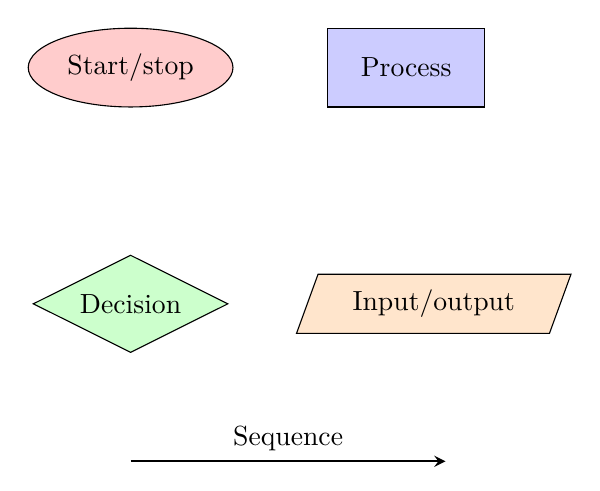
\begin{tikzpicture}
                \node (startstop) [startstop] {Start/stop};
                \node (process) [process, right of=startstop, xshift=2.5cm] {Process};
                \node (decision) [decision, below of=startstop, yshift=-2cm] {Decision};
                \node (io) [io, below of=process, xshift=.35cm, yshift=-2cm] {Input/output};
                \draw [arrow] (0,-5) -- (4,-5) node[midway, above] {Sequence};
            \end{tikzpicture}
        \end{column}
        \end{columns}
    \end{frame}


    \begin{frame}{Example Flowchart: Factorial of a Number}
        \centering
        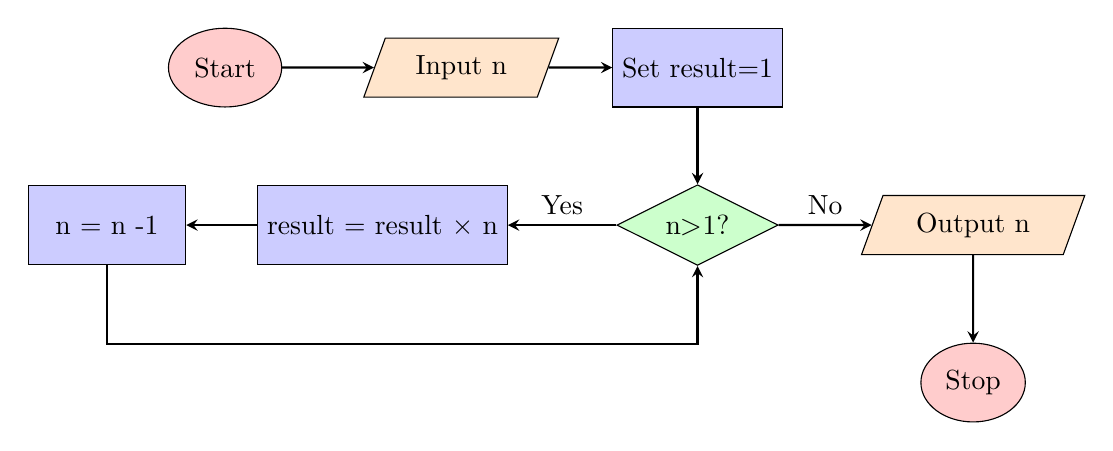
\begin{tikzpicture}%[node distance=2cm]
            \node (start) [startstop] {Start};
            \node (input) [io, right of=start, xshift=2cm] {Input n};
            \node (init_res) [process, right of=input, xshift=2cm] {Set result=1};
            \node (check_n) [decision, below of=init_res, yshift=-1cm] {n$>$1?};
            \node (upd_res) [process, left of=check_n, xshift=-3cm] {result = result × n};
            \node (upd_n) [process, left of=upd_res, xshift=-2.5cm] {n = n -1};
            \node (output) [io, right of=check_n, xshift=2.5cm] {Output n};
            \node (stop) [startstop, below of=output, yshift=-1cm] {Stop};

            \draw [arrow] (start) -- (input);
            \draw [arrow] (input) -- (init_res);
            \draw [arrow] (init_res) -- (check_n);
            \draw [arrow] (check_n) -- (upd_res) node[midway, above] {Yes};
            \draw [arrow] (upd_res) -- (upd_n);
            \draw [arrow] (upd_n.south) -- ++(0, -1) -| (check_n.south);
            \draw [arrow] (check_n) -- (output) node[midway, above] {No};
            \draw [arrow] (output) -- (stop);
        \end{tikzpicture}
    \end{frame}


    \section{Pseudocode}


    \begin{frame}{Purpose of Pseudocode}
        \begin{itemize}
            \item Represents algorithms in structured, human-readable code
            \item Independent of programming language, but may include programming key-words
            \item Easier to understand and refine before coding
        \end{itemize}
    \end{frame}


    \begin{frame}{Conventions}
        \begin{itemize}
            \item Indentation to show structure
            \item Keywords like IF, WHILE, FOR
            \item Use natural language mixed with structured logic
        \end{itemize}
    \end{frame}


    \begin{frame}[fragile]{Example pseudocode: Factorial of a Number}
        \begin{verbatim}
Input n
Set result = 1
While n>1:
    result = result * n
    n = n - 1
EndWhile
Output n
        \end{verbatim}
    \end{frame}


    \section{Control Structures}

    \begin{frame}{Sequence}
        \begin{itemize}
            \item Default mode of execution: step by step
            \item Example: Read number, calculate square, print result
        \end{itemize}
    \end{frame}


    \begin{frame}{Selection}
        \begin{itemize}
            \item \textbf{IF}: execute a block if condition is true
            \item \textbf{IF–ELSE}: choose between two alternatives
            \item \textbf{ELSE IF ladder}: multiple conditions
        \end{itemize}
    \end{frame}


    \begin{frame}{Iteration}
        \begin{itemize}
            \item \textbf{FOR loop} – fixed number of iterations
            \item \textbf{WHILE loop} – repeat while condition is true
            \item \textbf{DO–WHILE loop} – run at least once, then repeat if condition holds
        \end{itemize}
    \end{frame}


    \begin{frame}{While vs Do-While}
        \begin{columns}
        \begin{column}{0.5\textwidth}
            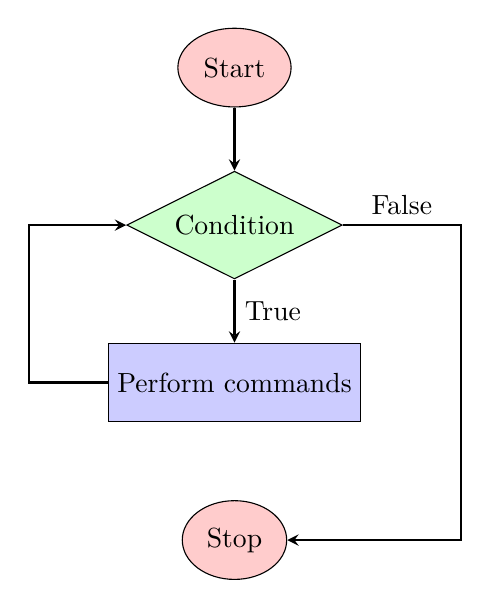
\begin{tikzpicture}
                \node (start) [startstop] {Start};
                \node (cond) [decision, below of=start, yshift=-1cm] {Condition};
                \node (command) [process, below of=cond, yshift=-1cm] {Perform commands};
                \node (stop) [startstop, below of=command, yshift=-1cm] {Stop};

                \draw [arrow] (start) -- (cond);
                \draw [arrow] (cond) -- (command) node[midway, right] {True};
                \draw [arrow] (command.west) -- ++(-1, 0) |- (cond);
                \draw [arrow] (cond.east) -- node[midway, above] {False} ++(1.5, 0) |- (stop);
            \end{tikzpicture}
        \end{column}
        \begin{column}{0.5\textwidth}
            \begin{tikzpicture}
                \node (start) [startstop] {Start};
                \node (command) [process, below of=start, yshift=-1cm] {Perform commands};
                \node (cond) [decision, below of=command, yshift=-1cm] {Condition};
                \node (stop) [startstop, below of=decision, yshift=-2cm] {Stop};

                \draw [arrow] (start) -- (command);
                \draw [arrow] (command) -- (cond);
                \draw [arrow] (cond.east) -- ++(1.5, 0) node[midway, above] {True} |- (command.east);
                \draw [arrow] (cond) -- (stop) node[midway, right] {False};
            \end{tikzpicture}
        \end{column}
        \end{columns}
    \end{frame}


    \begin{frame}{Break and Continue}
        \begin{itemize}
            \item \textbf{BREAK}: exit the nearest loop immediately (\texttt{exit} in Fortran)
            \item \textbf{CONTINUE}: skip rest of current iteration, proceed to next (\texttt{cycle} in Fortran)
        \end{itemize}
    \end{frame}


    \begin{frame}{Recursion}
        \begin{itemize}
            \item Function calling itself to solve smaller subproblems
            \item Example: factorial, Fibonacci
            \item Must have a base case to terminate
        \end{itemize}
    \end{frame}


    \begin{frame}[fragile]{Recursion Example: Factorial of a Number}
        \begin{verbatim}
Function Factorial(n):
    If (n==0):
        Return 1
    Else:
        Return n * Factorial(n-1)
    EndIf
EndFunction
        \end{verbatim}
    \end{frame}


    % \begin{frame}{Structured Programming Principles}
    % \begin{itemize}
    %     \item Every program can be built using the three structures (sequence, selection, and iteration)
    %     \item Avoids unstructured jumps like \texttt{goto}
    %     \item Easier to read and understand
    %     \item Easier to test and debug
    %     \item Encourages modular design and reuse
    % \end{itemize}
    % \end{frame}
    

    \begin{frame}{Best Practices}
    \begin{itemize}
        \item Keep flowcharts clean and uncluttered
        \item Use consistent symbols and indentation
        \item Pseudocode should be language-independent
        \item Algorithms should be logically ordered and unambiguous
    \end{itemize}
    \end{frame}
    

    \begin{frame}{Common Pitfalls}
    \begin{itemize}
        \item Overcomplicating flowcharts with too many details
        \item Ambiguous pseudocode (mixing multiple languages)
        \item Ignoring edge cases in algorithms
        \item Writing unstructured logic
    \end{itemize}
    \end{frame}
    

    \begin{frame}{Putting It All Together}
    \begin{block}{Example task}
    Compute the sum of all even numbers from 1 to N
    \end{block}
    \end{frame}


    \begin{frame}{Algorithm}
    \begin{enumerate}
        \item Read n
        \item Set sum = 0, i = 1
        \item While i <= n:
            \begin{itemize}
                \item If i is even, add i to Sum, else do nothing
                \item Add 1 to i
            \end{itemize}
        \item Print sum.
    \end{enumerate}
    \end{frame}


    \begin{frame}{Flowchart}
        \centering
        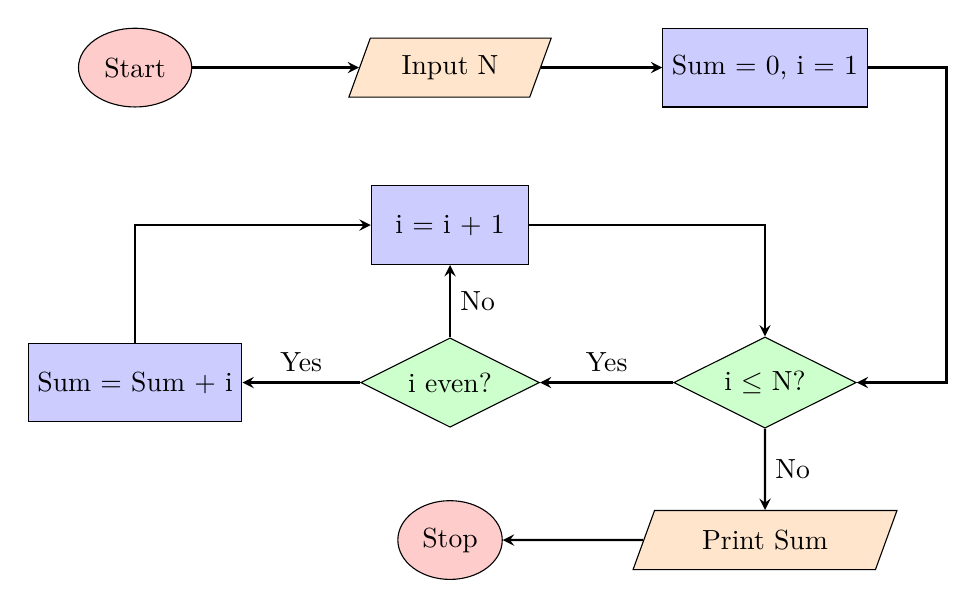
\begin{tikzpicture}[node distance=4cm]
            \node (start) [startstop] {Start};
            \node (in) [io, right of=start] {Input N};
            \node (init_sum_i) [process, right of=in] {Sum = 0, i = 1};
            \node (i_lt_n) [decision, below of=init_sum_i, yshift=-0cm] {i $\leq$ N?};
            \node (i_even) [decision, left of=i_lt_n] {i even?};
            \node (upd_sum) [process, left of=i_even, align=center] {Sum = Sum + i};
            \node (upd_i) [process, above of=i_even, yshift=-2cm] {i = i + 1};
            \node (out) [io, below of=i_lt_n, yshift=2cm] {Print Sum};
            \node (stop) [startstop, left of=out] {Stop};
            
            \draw [arrow] (start.east) -- (in.west);
            \draw [arrow] (in.east) -- (init_sum_i.west);
            \draw [arrow] (init_sum_i.east) -- ++(1,0) |- (i_lt_n.east);
            \draw [arrow] (i_lt_n.west) -- (i_even.east) node[midway,above] {Yes};
            \draw [arrow] (i_even.west) -- (upd_sum.east) node[midway,above] {Yes};
            \draw [arrow] (i_even.north) -- (upd_i.south) node[midway,right] {No};
            \draw [arrow] (upd_sum.north) |- (upd_i.west);
            \draw [arrow] (upd_i.east) -| (i_lt_n.north);
            \draw [arrow] (i_lt_n.south) -- (out.north) node[midway,right] {No};
            \draw [arrow] (out) -- (stop);
        \end{tikzpicture}
    \end{frame}


    \begin{frame}[fragile]{Pseudocode}
        \begin{verbatim}
Input n
sum = 0
i = 1
While (i <= n):
    If (i is even):
        sum = sum + i 
    EndIf
    i = i + 1
EndWhile
Output sum
        \end{verbatim}
    \end{frame}


    \section{Exercises}

    \begin{frame}{Exercises}
    \begin{enumerate}
        \item Design a algorithm and flow chart to find the largest of the three numbers
        \item Develop pseudocode for computing the sum of the digits of a given integer
        \item Write an algorithm and pseudocode to check whether a number is prime
    \end{enumerate}
    \end{frame}

    \section*{Questions?}
\end{document}
